\documentclass[preprint,12pt]{elsarticle}
\usepackage{amssymb}
\usepackage{graphicx}
\journal{Nuclear Instruments and Methods A}
\begin{document}
\begin{frontmatter}
\title{Electronics for Amplifying and Discriminating Veto Signals for MiniClean}
\author[mit]{R.~Abruzzio}
\author[mit]{B.~Buck\corref{cor1}}
\ead{bbuck@mit.edu}
\author[rhul]{J.~Monroe}
\author[mit]{K.~Pallidino}
\address[mit]{Massachusetts Institute of Technology, Cambridge, MA, USA}
\address[rhul]{Royal Holloway University of London, Egham, Surrey, UK}
\cortext[cor1]{Corresponding Author}
\begin{abstract}
For the MiniClean project being installed at SNOLAB in Sudbury Ontario, we designed the front end electronics to time multiplex 42 photomultiplier channels into 6 digitizer channels for the Veto System.  In addition, the system provides an "N Hit" signal with an amplitude proportional to the number of channels above a programmable threshold.  The system has three primary components.  The first is an Amplifier Discriminator card which provides the PMT bias, amplifies the analog signals, and also generates a signal proportional to the number of channels above a discriminator threshold.  The outputs are fed into delay lines made of standard coaxial cable to delay the signals by 50ns to 350ns.  These delay lines feed into the summer cards which make an analog sum of all of the input channels.  Due to low occupancy, this summer input becomes a time multiplexed version of 8 input channels.  This is then fed into the digitizers and DAQ system.  All of the "N Hit" signals are summed as well to provide a system wide "N Hit" signal which can be read out by the same DAQ electronics.
\end{abstract}

\begin{keyword}
keyword1 \sep keyword2 \sep keyword3
\end{keyword}

\end{frontmatter}

\section{Introduction}
\label{Introduction}
The MiniClean project is a detector searching for WIMP dark matter using a liquid Argon target material.  The detector is located 6800 feet underground in the Cube Hall at SNOLAB in Sudbury, Ontario.  The detector consists of a sphere of liquid Argon or Neon surrounded by optical sensors inside a cryostat.  The Cryostat is submerged in water tank which provides additional background shielding as well as a veto function.  The water acts as a scintillation material for Muons which could create a signal in the detector.  48 PMTs inside the water volume will detect Muons and trigger a veto signal.  We describe the electronics to Bias the PMTs, Time Multiplex 8 PMT channels into a single digitizer channel, and generate a signal proportional to the number of PMTs above threshold at any moment.  An overview of the system is shown in Figure~\ref{fig:block_diagram}.

\begin{figure}[h]
\begin{center}
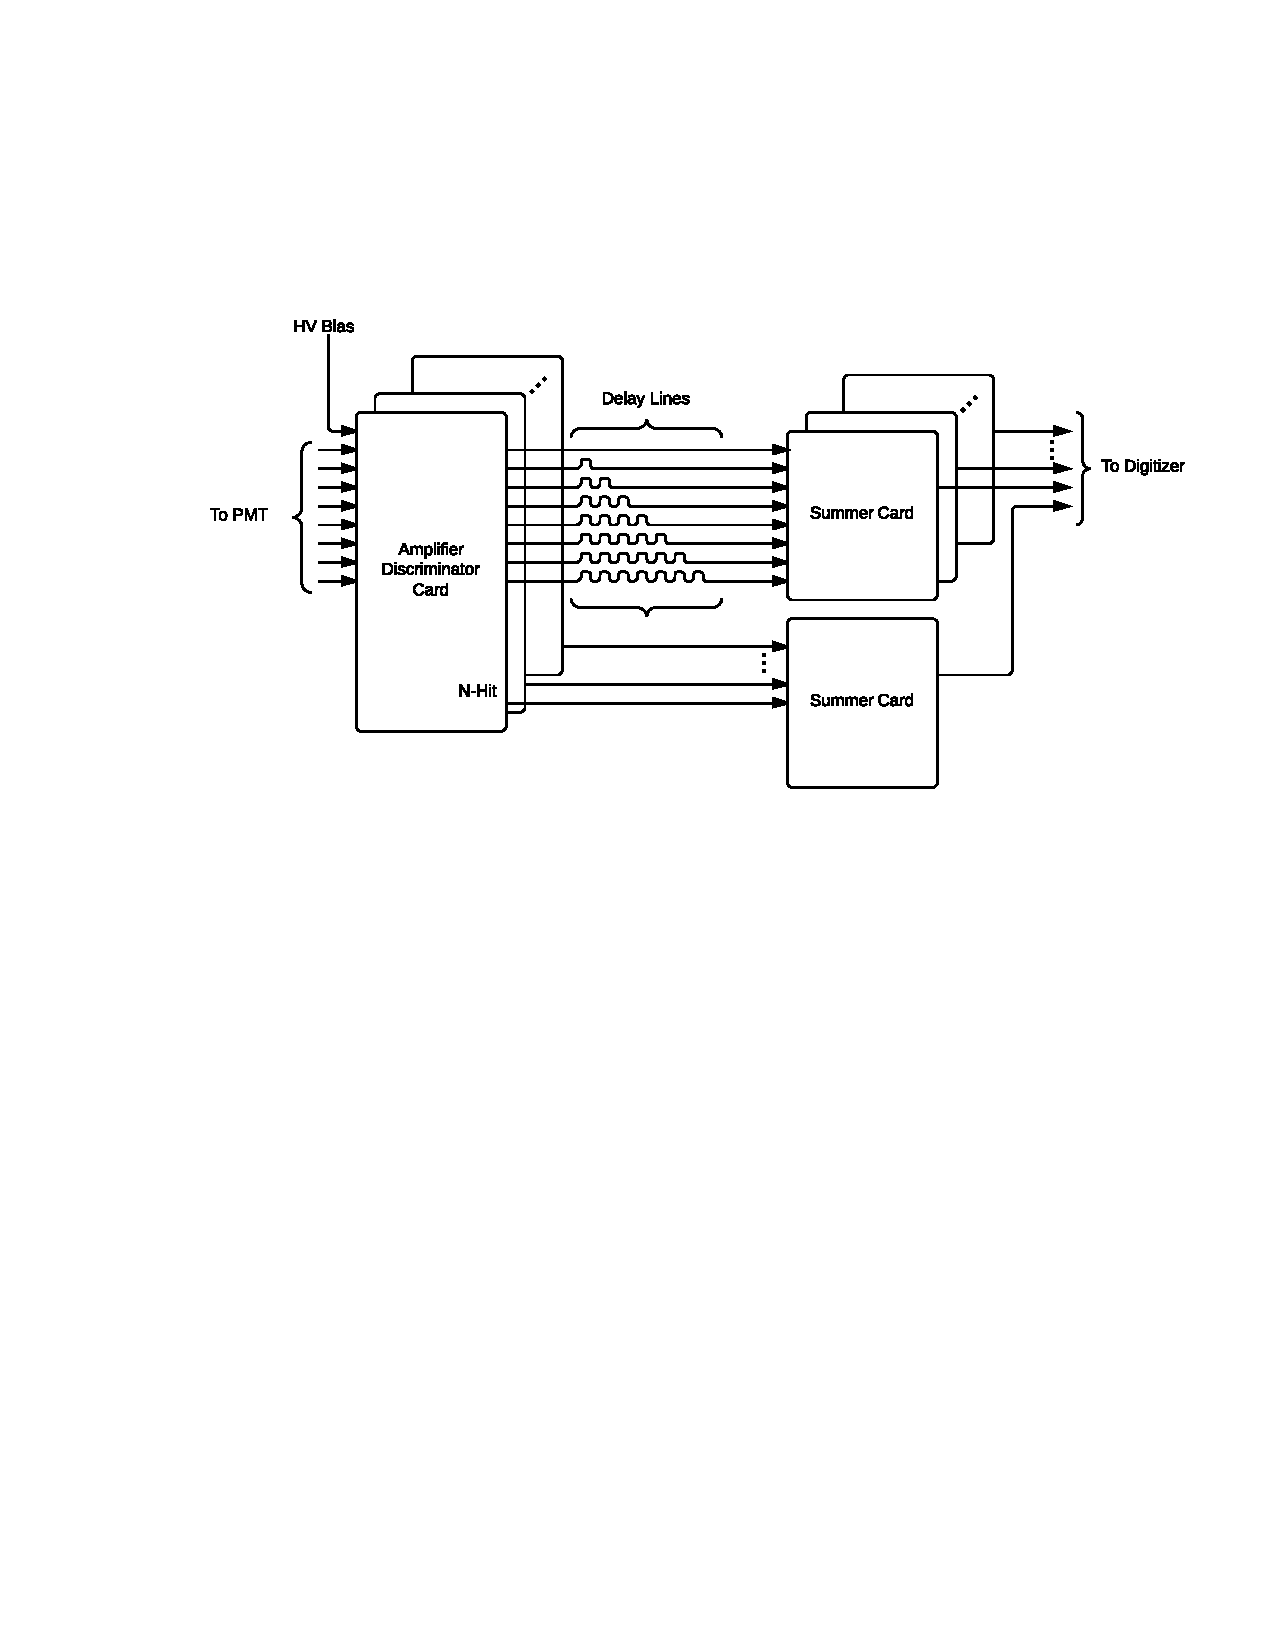
\includegraphics[width=5in, keepaspectratio=true, trim=1.25in 5.75in 0.5in 2in, clip=true]{graphics/block}
\caption{Block Diagram of MiniClean Veto Electronics}
\label{fig:block_diagram}
\end{center}
\end{figure}

\section{Amplifier Discriminator Board}
\label{Amp-Disc}
The Amplifier Discriminator Board is the front end electronics board.  The board provides high voltage distribution to the PMTs, signal amplification, and signal discrimination for the N Hit Sum.  The PMT bias voltage is fed to each of the PMT connections through a single SHV connector.  Each PMT capicatively couples the signal onto the bias voltage line.  On the Amplifier Discriminator board each channel has an amplifier input capacitvely coupled to the bias voltage line.  The PMT bias scheme is shon in Figure~\ref{fig:bias}.

\begin{figure}[h]
\begin{center}
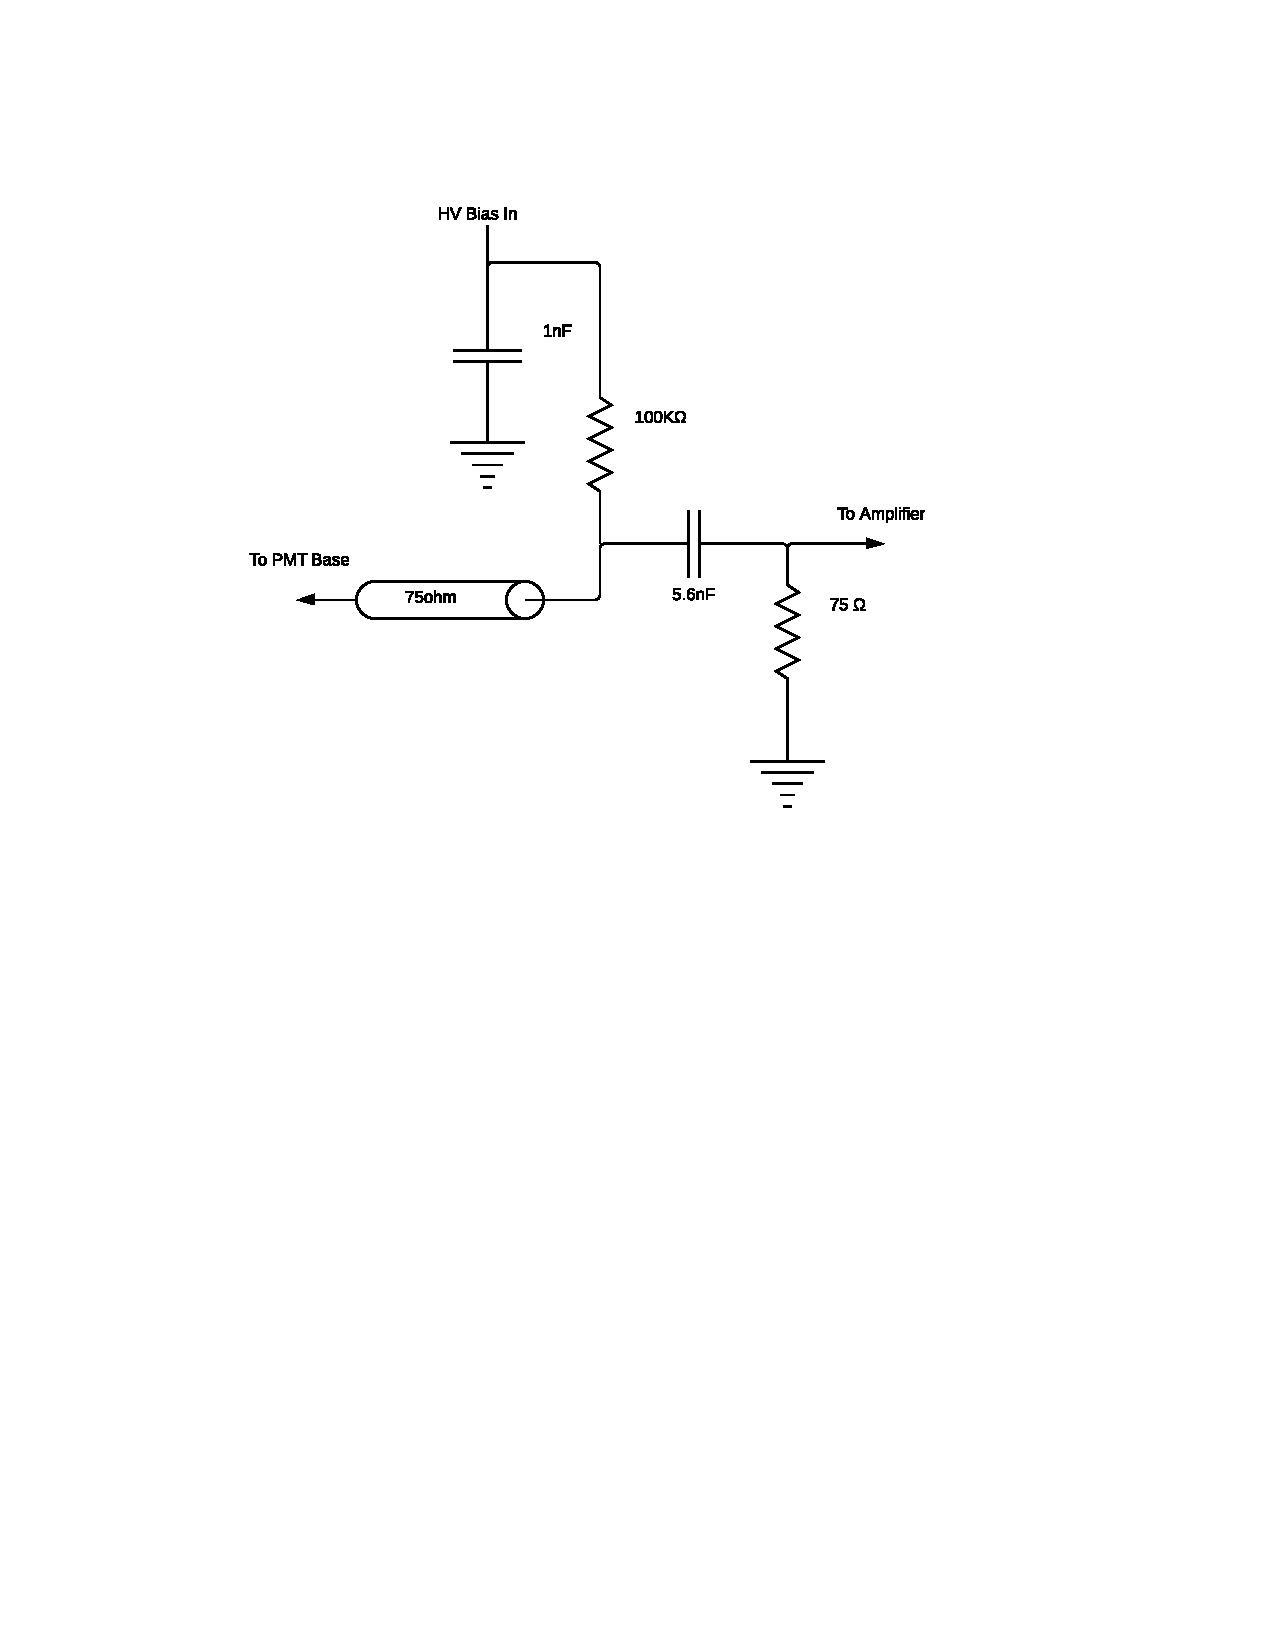
\includegraphics[width=3in, keepaspectratio=true, trim=1.5in 5.5in 2in 1.25in, clip=true]{graphics/bias}
\caption{Bias-T Schematic}
\label{fig:bias}
\end{center}
\end{figure}

The HV bias components were surface mount types.  Because of the aspect ratio of the width and length of some of the components, the components had to be raised slightly off of the board during the soldering process to ensure that flux could be cleaned from underneath the components.  In addition, the HV components were potted with corona dope.

A high bandwidth Current Feedback Amplifier (CFA) provides the large gain and bandwidth needed to amplify the pulses in a single stage.  We selected the Analog Devices AD8000 CFA to amplify the PMT pulses.  The amplified pulses are fed through out to the delay lines and to the discriminator comparators.  Due to the high-gain requirements, and the variations between the CFAs, all of the parts installed were tested beforehand and binned into parts with a similar DC offset.  During board assembly, care was taken to ensure that all of the amplifiers installed on a single board had a similar DC offset.

The comparator compares each channel with a programmable threshold voltage, common to all 8 channels on each board.  The output of the comparator is a fast differential PECL output.  These are summed with a differential amplifier and output using a transformer as a single ended signal, the "N-Hit sum" for those 8 channels.

The Amplifier Discriminator Board has local linear power regulation.  Each board has two +5V supplies, one -5V supply, and one +3V supply.  The CFA runs on the +5V and -5V supplies.  The comparator runs on the second +5V supply and the +3V supply (necessary for PECL output).  There are two +5V supplies in order to isolate the output supply for the comparator in order to reduce cross talk.  The regulators are fed by a common bipolar supply and ground nominally at $\pm$ 9V.  The nominal values for current draw are 500mA on the positive rail and 250mA on the negative rail.

The board is constructed with 4 copper layers and standard FR4 substrate material, with 0.062" thickness.  It is mounted on a piece of FR4 to protect HV nets on the bottom of the board from arcing and to fit it into a 6U VME style crate.  9 SHV connectors are mounted on a front panel connected to the FR4 and provide the HV Bias Input and eight PMT connections.  These PMT connections attach on the left side of the board with short HV insulated wire pig tails.  On the right side of the board 9 SMA connectors are board mounted.  The SMA connectors provide the eight signal outputs to the delay lines and the one N-Hit sum signal.

\section{Delay Lines}
\label{Delay}
The delay lines connect from the Amplifier Discriminator boards to the Summer Boards.  They are designed to delay the signals 50nS to 350nS.  Since the expected signals have a very low occupancy (!!!what is the occupancy) and the pulses are expected to be short in comparison to the 50nS delay window, delaying the signals and summing them together has the effect of time multiplexing the signals.  The delay lines are made of different lengths of Belden 9310 cable fitted with male SMA connectors.  The cable was chosen for its low attenuation, slow signal propagation speed, and small bend radius.  There are 7 different lengths ranging form 32' to 224', with every 32' equating to about 50 nS of delay.  These are coiled inside a metal box with pig tails to connect to the Amplifier Discriminator Boards and the Summer Boards.  The metal box satisfies fire protection concerns in the mine, as the Belden 9310 is not plenum rated.  There are two sets of each of the seven lengths in each box.  Of course, one of the signals should have a 0nS delay and is connected from the Amplifier Discriminator card to the summer card with a very short jumper cable.

\section{Summer Board}
\label{Sum}
The Summer Board sums the analog channels after they have been delayed, and also sums the N Hit Sums from each of the 6 cards to make a global N Hit Sum.  The Summer Board has 8 inputs, female SMA connectors.  Each of these inputs is fed, DC coupled, into a CFA to provide buffering.  This also provides the opportunity to fine tune the gain and equalize the signals after the cable delay by adjusting the two feedback resistors.  the outputs are fed into another CFA configured as an analog summing node.  This outputs through a series resistor to an female MCX connector.  A short jumper cable will connect the Summer Board output to the digitizer input.
Like the Amplifier Discriminator Board, the Summer Board has local power regulation.  Each board has one +5V supply and one -5V supply.  The regulators are fed by a common bipolar supply with ground between $\pm$ 7V to $\pm$ 12V.  The nominal values for current draw are 250mA on the positive rail and 250mA on the negative rail.

\begin{figure}[h]
\begin{center}
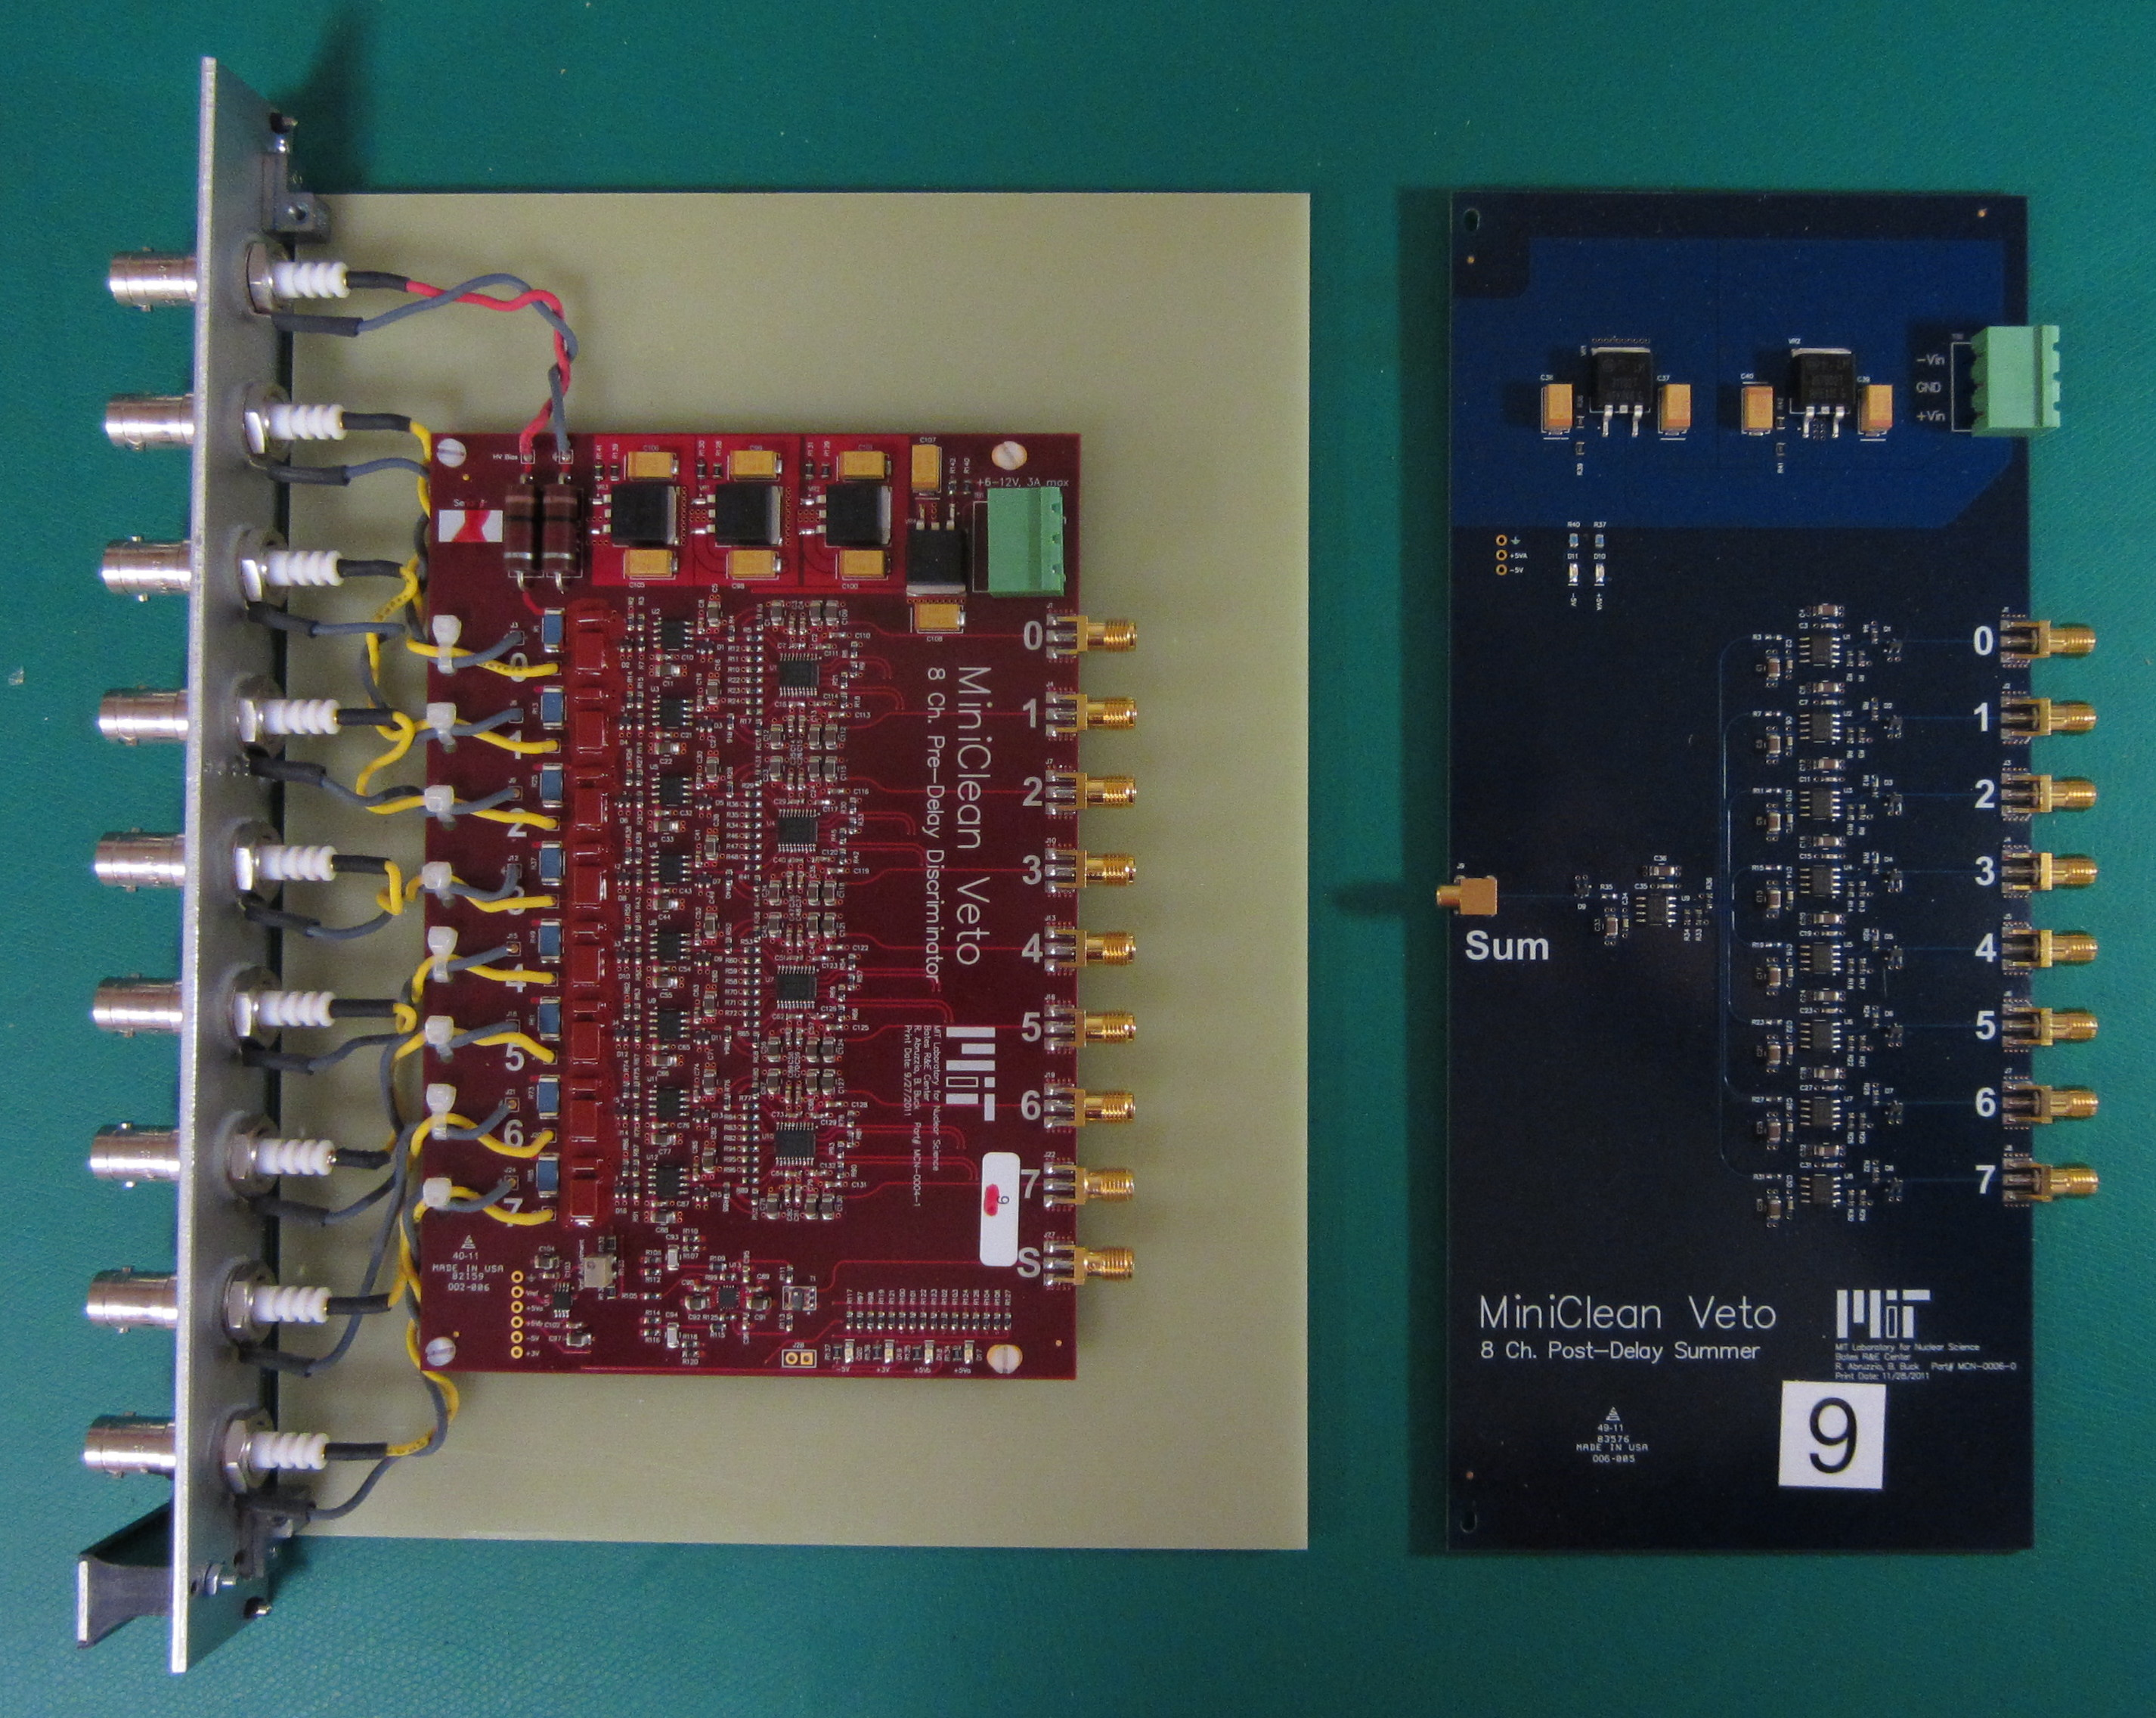
\includegraphics[width=5in, keepaspectratio=true]{graphics/boards}
\caption{Amplifier Discriminator Board (left) and Summer Board (right)}
\label{fig:boards}
\end{center}
\end{figure}

\section{Housing and Assembly}
\label{Housing}
The electronics are housed in a rack which holds a crate for the electronics, a fan unit for cooling, a power supply unit, and all of the delay lines.  The power supply module provides $\pm$ 9V up to 130W.  Estimated total power draw is 72W.  The power supply uses two discrete 9V switching power supplies which provide +9, 0, and -9 V power rails running on the back of the rack.  Connectors are attached to these rails and insert into each of the electronics boards.  Each of the components was tested individually at MIT.  Amplifier Discriminator boards were high-pot tested and all channels were tested to ensure uniformity.  Summer channels were similarly tested.  The boards were assembled into a VME style crate and mounted in a rack together with the power supply unit, the fan unit, and the delay lines.  An integration test was done at Boston University to demonstrate the system running while attached to the data acquisition system.

\section{Summary}
\label{Summary}
During testing we were able to demonstrate the system working properly.  We were able to see simulated events pushed into the system and see the N Hit signal increase proportional to the number of PMTs which were hit.  We could observe the output signals on the time multiplexed outputs from the summer boards.  Once operational, the full system will multiplex 48 PMT signals into 6 digitizer channels and provide a system wide N Hit sum.  The system is now at SNOLAB (???!!!) ready for implementation in the experiment.

\end{document}
